\documentclass{article}
\usepackage{tikz}
\usepackage{pgfplots}

\begin{document}

\begin{figure}[h]
    \centering
    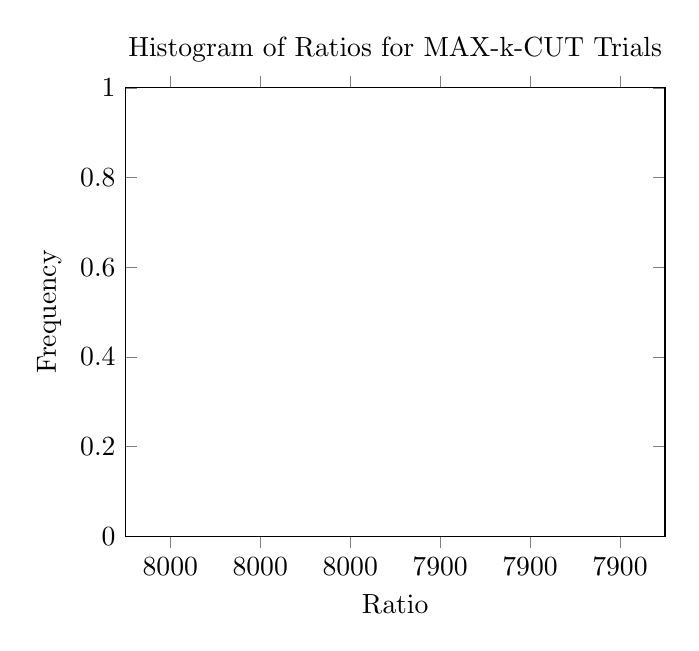
\begin{tikzpicture}
        \begin{axis}[
            ybar,
            symbolic x coords={8000, 7900, 7800, ..., 10},
            xtick=data,
            ymin=0,
            ymax=500,
            ylabel={Frequency},
            xlabel={Ratio},
            title={Histogram of Ratios for MAX-k-CUT Trials}
        ]
            % Add data points here
            % For example:
            % \addplot coordinates {(8000, 200) (7900, 150) ...};
        \end{axis}
    \end{tikzpicture}
    \caption{Histogram of Ratios for MAX-k-CUT Trials}
\end{figure}

\end{document}